

\chapter{Linear Discrete Maps}
%
% \section{Modeling with Discrete Maps}
%
% \emph{To do:} Introduce modeling with maps;
% define the \emph{order}\index{order} of a map; ...
\section{One-Dimensional Maps}
\label{sec:OneDimMaps}
We begin with the simplest model of population growth.
Suppose, for example, a population increases by 15 percent each
year.
Let $p(n)$ be the population at the end of year $n$, and assume that
$p(0)$ is given.
Then an increase of 15 percent each year gives
\begin{equation}
  p(n+1) = 1.15p(n).
  \label{eqn:pop}
\end{equation}
If $p(0)=100$, then $p(1) = 1.15(100) = 115$,
$p(2) = 1.15(115) = 132.3$, $p(3) = 1.15(132.3) = 152.1$, and so on. 
Table~\ref{tbl:popdata} shows the first nine iterations of
this process.
The data is plotted in Figure~\ref{fig:popdataplot}.
\begin{table}[h]
\centerline{%
\begin{tabular}{|c|l|c|l|}
\hline
 $n$  &  $p(n)$ & $n$ & $p(n)$ \\ 
\hline
  0  & 100.0  & 5 & 201.1 \\ 
\hline
  1 &  115.0  & 6 & 231.3 \\ 
\hline
  2 &  132.3  & 7 & 266.0 \\ 
\hline
  3 &  152.1  & 8 & 305.9\\ 
\hline
  4 &  174.9  & 9 & 351.8 \\ 
\hline
\end{tabular}
\vspace{0.25cm}
}
\caption{Iteration of the map~\eqref{eqn:pop}, with
$p(0)=100$.}
\label{tbl:popdata}
\end{table}

\begin{figure}
\centerline{%
\includegraphics[width=3.25in]{matlab_map1d/popdataplot.eps}
}
\caption{Plot of the data for the simple population growth
model~\eqref{eqn:pop}.  The data is in Table~\ref{tbl:popdata}.}
\label{fig:popdataplot}
\end{figure}

We derive a formula for $p(n)$ by noting that
\begin{equation}
\begin{split}
   p(1) & = 1.15p(0) \\
   p(2) & = 1.15p_1 = (1.15)^2 p(0) \\
   p(3) & = 1.15p_2 = (1.15)^3 p(0) \\
       & \vdots \\
   p(n) & = (1.15)^n p(0)
\end{split}
\end{equation}
Thus we have the familiar ``exponential growth'' of the
population.

More generally, the same argument shows that the solution
to
\begin{equation}
   p(n+1) = a p(n),
\end{equation}
given $p(0)$, is
\begin{equation}
   p(n) = a^k p(0).
\label{eqn:psol}
\end{equation}

Let's compare the discrete time map to the continuous time model.
Recall that a first order differential equation
that leads to exponential growth
(or decay) is
\begin{equation}
 \frac{dp}{dt} = r p, \quad\quad p(0) = p_0,
\label{eqn:contpop}
\end{equation}
which has the solution
\begin{equation}
  p(t) = p_0e^{rt} = \left( e^r\right)^t p_0.
\end{equation}
I've written the solution as
$\left(e^r\right)^t p_0$ to make clear the analogy
between the continuous solution and the solution to the discrete
model in \eqref{eqn:psol}.
The term $e^r$ is analogous to $a$, and $t$ is analogous to $n$.

Let's rewrite \eqref{eqn:pop} as
\begin{equation}
  p(n+1) = (1 + 0.15)p(n) = p(n) + 0.15p(n)
\end{equation}
or
\begin{equation}
  p(n+1) - p(n) = 0.15p(n) .
\end{equation}
This form of the equation expresses the
\emph{discrete change} in
$p(n)$ as a function of $p(n)$.
(Such an equation is often called a \emph{difference equation}.)
Compare this to equation~\eqref{eqn:contpop}, which gives the
\emph{instantaneous rate of change} of $p$ as a function
of $p$.


%\newpage
% \subsection*{Linear Maps}
% 
% A \emph{linear} one-dimensional map is
% \begin{equation}
%    x_{n+1} = a x_n
% \end{equation}
% where $a$ is a constant.
% (The population model \eqref{eqn:pop}
% is an example.)
% The solution is
% \begin{equation}
%    x_n = a^n x_0.
% \end{equation}
Consider how the behavior of the solution
to \eqref{eqn:psol} depends on $a$.
\begin{itemize}
\item If $a > 1$, then $a^n > 0$, and $a^n$ increases without
bound as $n$ increases. So $p(n)$ grows exponentially.
\item If $a = 1$, then $a^n=1$ for all $n$, so $p(n) = p(0)$.
\item If $0 < a < 1$, then $a^n > 0$, and $a^n$ approaches
zero as $n$ increases; $p(n)$ decays to zero monotonically.
\item If $a=0$, then $p(n)=0$ for all $n > 0$.
\item If $-1 < a < 0$, then $a^n$ alternates sign, and
$a^n$ approaches zero as $n$ increases;
$p(n)$  decays to zero while alternating sign.
\item If $a = -1$, then $a^n = (-1)^n$, which is $1$ if $n$
is even and $-1$ if $n$ is odd.  Thus $p(n)$ alternates
between $p(0)$ and $-p(0)$.
\item If $a < -1$, then $a^n$ alternates sign,
and $|a^n|$ increases without bound as $n$ increases.
So $p(n)$ alternates sign while $|p(n)|$ grows exponentially.
\end{itemize}
Overall, the magnitude of $p(n)$ \emph{grows if} $|a| > 1$,
and \emph{decays if} $|a| < 1$.
Figures~\ref{fig:linearcases_pos}
and \ref{fig:linearcases_neg} show sample plots of $p(n)$
% and cobweb diagrams
for the various cases.
\begin{figure}
\centerline{%
\includegraphics[width=4.25in]{matlab_map1d/linearcases_pos.eps}
}
\caption{Examples of linear maps, $a \ge 0$. In all cases, $p(0)=10$.}
\label{fig:linearcases_pos}
\end{figure}
%
\begin{figure}
\centerline{%
\includegraphics[width=4.25in]{matlab_map1d/linearcases_neg.eps}
}
\caption{Examples of linear maps, $a < 0$. In all cases, $p(0)=10$.}
\label{fig:linearcases_neg}
\end{figure}
%

\newpage
\section{Two-Dimensional Maps}

We consider the linear maps of the plane
\begin{equation}
\begin{split}
  x(n+1) & = a_{11}x(n) + a_{12}y(n) \\
  y(n+1) & = a_{21}x(n) + a_{22}y(n)
\end{split}
\end{equation}
with a given starting point $(x_0,y_0)$,
or equivalently,
\begin{equation}
  \BX(n+1) = A\BX(n), \quad \textrm{where} \quad
     \BX(n) = \begin{bmatrix} x(n) \\ y(n) \end{bmatrix},
     \quad
     A = \begin{bmatrix} a_{11} & a_{12} \\ a_{21} & a_{22} \end{bmatrix},
\label{eqn:linearmap}
\end{equation}
and the starting vector is
$\ds \BX(0) = \BX_0 = \begin{bmatrix} x_0 \\ y_0 \end{bmatrix}$.
%
%
\subsection*{Solving the System}
We note if $\BX_0 = \begin{bmatrix}0 \\ 0\end{bmatrix} \equiv \BZero$, then $\BX(n) = \BZero$ for all $n>0$ is a solution to \eqref{eqn:linearmap}.
Such a constant solution is called a \emph{fixed point}\index{fixed point}
of the map.

More generally, we can ``solve'' this system by simply iterating the
map:
\begin{equation}
\begin{split}
  \BX(1) & = A\BX_0 \\
  \BX(2) & = A\BX(1) = A^2\BX_0 \\
  \BX(3) & = A\BX(2) = A^3\BX_0 \\
        & \vdots \\
  \BX(n) & = A^n\BX_0
\end{split}
\end{equation}
This is a solution, but it doesn't tell us much about the
behavior of the solutions.  A lot of information is hidden
in $A^n$.

An alternative approach is to use a procedure similar to the
method we used to solve linear systems of differential equations.
In the case of a linear map, we propose a solution of the
form
\begin{equation}
   \BX(n) = \lambda^n \BV
\label{eqn:solutionguess}
\end{equation}
where $\lambda$ is a number and $\BV$ is a constant vector.
We already know that $\BX(n)\equiv\BZero$ is a solution, so without
loss of generality we assume that $\lambda\ne 0$ and
$\BV \ne \BZero$.

By substituting this ``guess'' into \eqref{eqn:linearmap},
we obtain
\begin{equation}
  \lambda^{n+1} \BV  = A\lambda^n\BV
\end{equation}
or, after canceling a factor of $\lambda$ and rearranging,
\begin{equation}
   A\BV = \lambda \BV.
\label{eqn:mapeigenvalueprob}
\end{equation}
This is the familiar \emph{eigenvalue problem}\index{eigenvalue problem}
for the matrix $A$.
To solve \eqref{eqn:linearmap}, we must find
the eigenvalues ($\lambda$) and
the corresponding eigenvectors ($\BV$) of $A$.
If $\lambda$ is an eigenvalue of $A$ and $\BV$ is a corresponding
eigenvector, then~\eqref{eqn:solutionguess} is a solution
to~\eqref{eqn:linearmap}.

Let's consider what such a solution looks like in the
$(x,y)$ plane.  Consider, for example,
\begin{equation}
   A = \begin{bmatrix} 1 & \frac{1}{2} \\
                      \frac{3}{4} & \frac{5}{4}
       \end{bmatrix}
\label{eqn:example1}
\end{equation}
The eigenvalues of $A$ are $\lambda_1 = \frac{1}{2}$
and $\lambda_2 = \frac{7}{4}$,
with eigenvectors $\BV_1 = \begin{bmatrix} 1 \\ -1 \end{bmatrix}$
and $\BV_2 = \begin{bmatrix} 2 \\ 3 \end{bmatrix}$, respectively.
So two solutions are $(1/2)^n\BV_1$ and $(7/4)^n\BV_2$.
The plot on the left in
Figure~\ref{fig:Lin2DMapExample1} shows the first three iterations
of the solutions $(1/2)^n\BV_1$.  Since
$(1/2)^n\rightarrow 0$ and $n$ increases, further iterations
will converge to the origin.
\begin{figure}
\centerline{%
\includegraphics{matlab/Lin2DMapExampleEig.eps}
\includegraphics{matlab/Lin2DMapExample1.eps}
}
\caption{%
The plot on the left shows several iterations of the
solution $\BX(n) = \lambda_1^n\BV_1$ of the linear map
for $A$ given in \eqref{eqn:example1}.
The trajectory begins at
$\BX_0 = \BV_1$.
The plot on the right shows several more trajectories
of the same system.
}
\label{fig:Lin2DMapExample1}
\end{figure}
The iterates in the second solution, $(7/4)^n\BV_2$,
remain on the line $y=(3/2)x$, but in this case they move further
and further \emph{away} from the origin, since $7/4 > 1$.


Because the map is linear, we can form the \emph{general solution}
by taking linear combinations of these two special solutions.
That is, at least when $\lambda_1$ and $\lambda_2$ are real and
distinct eigenvalues, the general solution is
\begin{equation}
   \BX(n) = c_1 \lambda_1^n \BV_1 + c_2 \lambda_2^n \BV_2.
\end{equation}
The constant $c_1$ and $c_2$ are chosen so that
the initial condition is satisfied. That is, 
\begin{equation}
   c_1 \BV_1 + c_2 \BV_2 = \BX_0.
\end{equation}


Figure~\ref{fig:Lin2DMapExample1} shows several trajectories
of the map with $A$ given in \eqref{eqn:example1}.
The trajectories shown in Figure~\ref{fig:Lin2DMapExample1}
might suggest that the trajectories of linear maps
behave the same as trajectories of
linear systems of  differential equations,
only with discrete jumps instead of smooth curves.
However, maps actually have more possible behaviors.
Consider, for example, the map with
\begin{equation}
  A = \begin{bmatrix} 1 & -\frac{1}{2} \\
                  -\frac{3}{4} & -\frac{1}{4}
      \end{bmatrix}
\label{eqn:example2}
\end{equation}
This matrix has eigenvalues $\lambda_1 = -\frac{1}{2}$ and
$\lambda_2 = \frac{5}{4}$, with eigenvectors
$\BV_1 = \begin{bmatrix} 1/3 \\ 1\end{bmatrix}$
and $\BV_2 = \begin{bmatrix} -2 \\ 1 \end{bmatrix}$, 
respectively.
The first few iterations of the solution $\lambda_1^n \BV_1$
are shown on the left in Figure~\ref{fig:Lin2DMapExample2}.
Because $\lambda_1 < 0$, $\lambda_1^n$ alternates sign, and the
trajectory jumps from one side of the origin to the other
as $n$ increases.
\begin{figure}
\centerline{%
\includegraphics{matlab/Lin2DMapExampleEigNeg.eps}
\includegraphics{matlab/Lin2DMapExample2.eps}
}
\caption{%
The plot on the left shows several iterations of the
solution $\BX(n) = \lambda_1^n\BV_1$ of the linear map
for $A$ given in \eqref{eqn:example2}.
The trajectory begins at
$\BX_0 = \BV_1$.
The plot on the right shows two more trajectories
of the same system.
}
\label{fig:Lin2DMapExample2}
\end{figure}
Two more trajectories for this system are shown on the right
in Figure~\ref{fig:Lin2DMapExample2}.
Note that after a few iterations,
the contribution of $c_1\lambda_1^n\BV_1$
becomes very small (since $\lambda_1^n\rightarrow 0$),
and the solutions are eventually dominated by 
$c_2\lambda_2^n\BV_2$.  This means the trajectories
converge to the line $y=-x/2$ as $n$ increases,
and since $\lambda_2 > 1$, the iterations diverge
from $\BZero$ as $n$ increases.

\subsection*{Stability.}
Suppose the $2\times 2$ matrix $A$ has real and distinct eigenvalues
$\lambda_1$ and $\lambda_2$.
\begin{itemize}
\item If $|\lambda_1|<1$ and $|\lambda_2|<1$, then
$\BX(n)\rightarrow\BZero$ as $n$ increases.  We say
$\BZero$ is a \emph{sink} or \emph{attractor}; also
$\BZero$ is \emph{asymptotically stable}.
\item If one eigenvalue, say $\lambda_1$ has magnitude less than
one and the other has magnitude greater than one, then
we call $\BZero$ a saddle.  (Both the examples shown in
Figures~\ref{fig:Lin2DMapExample1} and \ref{fig:Lin2DMapExample2}
are saddles.) A saddle is \emph{unstable}, because there
are trajectories beginning arbitrarily close of $\BZero$ that
diverge from $\BZero$.
\item If $|\lambda_1|>1$ and $|\lambda_2|>1$, then
$\BZero$ is a \emph{source} or \emph{repellor}.  (Of course,
a source is also unstable.)
\end{itemize}
%
%
\subsection*{Complex Eigenvalues.}
Here we consider the solutions when the eigenvalues of
$A$ are complex.  Recall that complex eigenvalues of a $A$
matrix must occur as complex conjugate pairs.
The following discussion is similar to how
we developed real-valued solutions for linear systems
of differential equations with complex eigenvalues.
 
Let $\lambda_1=\mu + i\omega$,
with eigenvector $\BV_1 = \BA + i \BB$.
A \emph{complex-valued} solution is
$\BX(n) = (\lambda_1)^n\BV_1$.
We'll write this as the sum of a real and imaginary part;
the real and imaginary parts of this solution are also solutions,
so they will give us a \emph{real-valued} set of solutions
with which we can create the general solution.

Recall \emph{Euler's Identity}:\index{Euler's formula}
 $e^{i\theta} = \cos \theta + i \sin\theta$.
We use this to write
\begin{equation}
\begin{split}
  \mu + i \omega & = \sqrt{\mu^2+\omega^2}\,
                      \left(\frac{\mu}{\sqrt{\mu^2+\omega^2}} +
		            i \frac{\omega}{\sqrt{\mu^2+\omega^2}}\right) \\
	         & = r (\cos\theta + i \sin\theta) \\
		 & = r e^{i\theta}, 
\end{split}
\end{equation}
where $r = |\lambda_1| = \sqrt{\mu^2+\omega^2}$
and $\theta = \tan^{-1}\left(\frac{\omega}{\mu}\right)$.
(The \emph{magnitude} of a complex number
$\lambda_1=\mu+i\omega$ is $|\lambda_1|=\sqrt{\mu^2+\omega^2}$.
If we think of the complex number as the point $(\mu,\omega)$
in Cartesian coordinates, then $r$ and $\theta$ are the
polar coordinates of the point.)
Then
\begin{equation}
\begin{split}
  \lambda_1^n & = (re^{i\theta})^n  \\
              & = r^n e^{in\theta}  \\
	      & = r^n(\cos(n\theta) + i \sin(n\theta))
\end{split}
\end{equation}
and
\begin{equation}
\begin{split}
   \lambda_1^n\BV_1 & = r^n(\cos(n\theta) + i \sin(n\theta))(\BA+i\BB) \\
     & = r^n(\BA\cos(n\theta)-\BB\sin(n\theta)) +
          i r^n(\BA\sin(n\theta)+\BB\cos(n\theta))
\end{split}
\end{equation}
The real and imaginary parts of this solution are
\begin{equation}
  u(n) = r^n(\BA\cos(n\theta)-\BB\sin(n\theta))
  \quad \textrm{and} \quad
  w(n) = r^n(\BA\sin(n\theta)+\BB\cos(n\theta)),
\end{equation}
respectively.
Each of these is solution to the linear map, and
we can use these to write the general solution as
\begin{equation}
  \BX(n) =    c_1 r^n(\BA\cos(n\theta)-\BB\sin(n\theta))
           + c_2 r^n(\BA\sin(n\theta)+\BB\cos(n\theta))
\end{equation}
Note that the terms in parentheses give vectors that
rotate by $\theta$ for each increase of $n$ by one.
We have the following possibilities
for the behavior of $\BX(n)$:
\begin{itemize}
\item
If $r < 1$, then $r^n \rightarrow 0$ as $n$ increases,
and therefore $\BX(n)\rightarrow \BZero$.
In this case, we say that $\BZero$ is a \emph{spiral sink}.
An example is shown on the left in Figure~\ref{fig:Lin2DMapExampleComplex1}.
\item
If $r=1$, then in the long run $\BX(n)$ does not approach
$\BZero$ or go off to infinity. Instead, it remains on an ellipse.
(However, $\BX(n)$ is \emph{not} periodic unless
$\frac{\theta}{2\pi}$ is a rational number.)
When $r=1$ we say that $\BZero$ is a \emph{center}.
Examples are shown in Figure~\ref{fig:Lin2DMapExampleComplexrz}.
\item
If $r > 1$, then $r^n$ grows exponentially, so $\BX(n)$
spirals away from the origin.  We say that $\BZero$ is 
a \emph{spiral source}.
An example is shown on the right in 
Figure~\ref{fig:Lin2DMapExampleComplex1}.
\end{itemize}

\begin{xexample}
We consider the system with
\begin{equation}
  A = \begin{bmatrix} 1/2 & -1/2\\ 1/2 & 1/2\end{bmatrix}.
\end{equation}
We find $\lambda = 1/2 \pm i/2$, and $r = \sqrt{1/2} < 1$.
The origin is a spiral sink.
See the plot on the left in Figure~\ref{fig:Lin2DMapExampleComplex1}.
\end{xexample}

\begin{xexample}
\begin{equation}
  A = \begin{bmatrix} 1/2 & -3/2\\ 3/2 & 1\end{bmatrix}.
\end{equation}
We find $\lambda = 3/4 \pm i\sqrt{35}/4$, and $r = \sqrt{11/4} > 1$.
The origin is a spiral source.
See the plot on the right in Figure~\ref{fig:Lin2DMapExampleComplex1}
\end{xexample}

\begin{xexample}
\begin{equation}
A = \begin{bmatrix} 13/15 & 8/15 \\ -4/3 & 1/3 \end{bmatrix}.
\end{equation}
We find $\lambda = \frac{3}{5}\pm \frac{4}{5}i$, $r=1$,
and $\theta = \tan^{-1}(4/3)\approx 0.9273$ radians.
Since $\theta$ is not a rational multiple of $2\pi$,
the iterates $\BX(n)$ will never repeat.
The first few iterations of a solution are shown
on the left
in Figure~\ref{fig:Lin2DMapExampleComplexrz}
\end{xexample}

\begin{xexample}
\begin{equation}
A = \frac{1}{6}\begin{bmatrix} 3+\sqrt{3} & 2\sqrt{3}\\ -5\sqrt{3} &  3-\sqrt{3}\end{bmatrix},
\end{equation}
We find $\lambda = 1/2 \pm i\sqrt{3}/2$, $r = 1$, and
$\theta=\pi/3$.
Since $6\theta = 2\pi$, solutions repeat after six iterations.
See the plot on the right in Figure~\ref{fig:Lin2DMapExampleComplexrz}.
\end{xexample}



\begin{figure}
\centerline{%
\includegraphics{matlab/Lin2DMapExampleComplex1.eps}
\includegraphics{matlab/Lin2DMapExampleComplex2.eps}
}
\caption{%
Examples with complex eigenvalues.
On the left:
%$A = \begin{bmatrix} 1/2 & -1/2\\ 1/2 & 1/2\end{bmatrix}$,
$\lambda = 1/2 \pm i/2$, $r = \sqrt{1/2} < 1$.
On the right:
%$A = \begin{bmatrix} 1/2 & -3/2\\ 3/2 & 1\end{bmatrix}$,
$\lambda = 3/4 \pm i\sqrt{35}/4$, $r = \sqrt{11/4} > 1$.
}
\label{fig:Lin2DMapExampleComplex1}
\end{figure}
%
\begin{figure}
\centerline{%
\includegraphics{matlab/Lin2DMapExampleComplexrz1.eps}
\includegraphics{matlab/Lin2DMapExampleComplexrz2.eps}
}
\caption{%
Examples with complex eigenvalues with $r=1$.
On the left,
%$A = \begin{bmatrix} 13/15 & 8/15 \\ -4/3 & 1/3 \end{bmatrix}$,
%$\lambda = \frac{3}{5}\pm \frac{4}{5}i$,
$\theta = \tan^{-1}(4/3)\approx 0.9273$ radians.
On the right,
%$A = \frac{1}{6}\begin{bmatrix} 3+\sqrt{3} & 2\sqrt{3}\\ -5\sqrt{3} &  3-\sqrt{3}\end{bmatrix}$,
%$\lambda = 1/2 \pm i\sqrt{3}/2$, $r = 1$,
$\theta=\pi/3$.
}
\label{fig:Lin2DMapExampleComplexrz}
\end{figure}

\newpage

\subsection*{Summary for the 2D Linear Maps.}
We summarize the general solution and stability results
for the two-dimensional linear maps~\eqref{eqn:linearmap}.
Let $\lambda_1$ and $\lambda_2$ be the eigenvalues of
$A$, with eigenvectors $\BV_1$ and $\BV_2$.
If the eigenvalues are complex, we assume
$\lambda_1 = \mu+i\omega$, where $\mu$ and $\omega$
are real numbers, and $\omega > 0$.  We also let $\BA$ and $\BB$
be the real vectors such that $\BV_1 = \BA+i\BB$.
We only consider the case in which the eigenvalues are distinct. 

\medskip
\noindent
\textbf{General Solution:}
\begin{itemize}
\item If the eigenvalues of $A$ are real and distinct, then the
general solution is
\begin{equation}
   \BX(n) = c_1 \lambda_1^n \BV_1 + c_2 \lambda_2^n \BV_2
\end{equation}
\item If the eigenvalues are complex, then
\begin{equation}
  \BX(n) =    c_1 r^n(\BA\cos(n\theta)-\BB\sin(n\theta))
           + c_2 r^n(\BA\sin(n\theta)+\BB\cos(n\theta))
\label{eqn:linear2dcomplexgensol}
\end{equation}
\end{itemize}

\noindent
\textbf{Stability:}
\begin{itemize}
\item If $|\lambda_1| < 1$ and $|\lambda_2| < 1$, then
$\BZero$ is a \emph{sink} or \emph{attractor}; it is
\emph{asymptotically stable}.
\item If either $|\lambda_1| > 1$ or $|\lambda_2|>1$, then
$\BZero$ is \emph{unstable}.
\item If both $|\lambda_1| > 1$ and $|\lambda_2|>1$, then
$\BZero$ is a \emph{source} or \emph{repellor}.
\end{itemize}

\medskip

\hrule

\medskip
\subsection*{Affine 2D Systems}
We point out here that it is no harder to solve the
system
\begin{equation}
  \BX(n+1) = A\BX(n) + \BG,
  \label{eqn:affine}
\end{equation}
where $\BG$ is a constant vector.
This is an example of a \emph{nonhomogeneous}
linear system.  It is also called an \emph{affine system}.

First, we find the fixed point $\BX^*$ of the map.
(In the following, we will assume that 
the matrix $A-I$ is invertible.  The case
where $A-I$ is singular is left as an exercise.)
The fixed point satisfies the equation
\begin{equation}
   A\BX^* + \BG  = \BX^*
\end{equation}
which we solve to find
\begin{equation}
   \BX^*  = -(A-I)^{-1}\BG.
\end{equation}
Define $\BY(n)$ so $\BX(n) = \BX^* + \BY(n)$,
and \eqref{eqn:affine} becomes
\begin{equation}
\begin{split}
  \BX^* + \BY(n+1) & = A\BX^* + A\BY(n) +\BG \\
  \BY(n+1) & = A\BY(n) + (A-I)\BX^* + \BG \\
            & = A\BY(n) + (A-I)\left(-(A-I)^{-1}\BG\right)+\BG \\
	    & = A\BY(n) -\BG+\BG \\
	    & = A\BY(n).
\end{split}
\end{equation}
So by changing coordinates to $\BY(n)$, we obtain
the linear system
\begin{equation}
  \BY(n+1) = A\BY(n) .
\end{equation}
We saw the same idea when we added a constant vector to a
linear system of differential equations.
Adding the constant vector to the right side of the equation
moves the equilibrium or fixed point, but
the dynamics around that point are the same
as the linear system without the constant vector added.

\newpage

\begin{exercises}
\begin{exercise}
For each of the following matrices, classify the
type and stability of the fixed point $\BZero$
for the discrete system $\BX(n+1) = A\BX(n)$.
\begin{enumerate}
\item[(a)]
$\ds A  =  \begin{bmatrix}
              0 & 1/2 \\
              1 & 0
           \end{bmatrix}$
\item[(b)]
$\ds A  =  \begin{bmatrix}
              1/4 & 0 \\
              1/2 & 1/2
           \end{bmatrix}$
\item[(c)]
$\ds A  =  \begin{bmatrix}
              3/5 & 1 \\
              -1/2 & 4/5
           \end{bmatrix}$
\item[(d)]
$\ds A  =  \begin{bmatrix}
              1 & 2 \\
              -1 & 3
           \end{bmatrix}$
\item[(e)]
$\ds A  =  \begin{bmatrix}
              1/4 & 1/4 \\
              -15/4 & 1/4
           \end{bmatrix}$
\item[(e)]
$\ds A  =  \begin{bmatrix}
              3 & -3 \\
              1/4 & 1
           \end{bmatrix}$
\end{enumerate}
\end{exercise}
\begin{exercise}
For each of the following, find the solution to the
system $\BX(n+1)=A\BX(n)$, $\BX(0)=\BX_0$.
\begin{enumerate}
\item[(a)]
$\ds A  =  \begin{bmatrix}
              0 & 1/2 \\
              1 & 0
           \end{bmatrix}$, \hspace*{.25cm} 
$\ds \BX_0 = \begin{bmatrix} 1 \\ 3 \end{bmatrix}$.
\item[(b)]
$\ds A  =  \begin{bmatrix}
              1/4 & 0 \\
              1/2 & 1/2
           \end{bmatrix}$, \hspace*{.25cm}
$\ds \BX_0 = \begin{bmatrix} -1 \\ 1 \end{bmatrix}$.
\item[(b)]
$\ds A  =  \begin{bmatrix}
              3/5 & 1 \\
              -1/2 & 4/5
           \end{bmatrix}$, \hspace*{.25cm} 
$\ds \BX_0 = \begin{bmatrix} 1 \\ 0 \end{bmatrix}$.
\end{enumerate}
\end{exercise}

\begin{exercise}
For each of the following affine systems, find the
fixed point and classify its type and stability.
\begin{enumerate}
\item[(a)] $\ds \BX(n+1) = \begin{bmatrix}
                         2 & 2 \\
                         1 & 2
                     \end{bmatrix}
                        \BX(n) + \begin{bmatrix} 3 \\ 1 \end{bmatrix}$
\item[(b)] $\ds \BX(n+1) = \begin{bmatrix}
                         2 & -2 \\
                         1 & 2
                     \end{bmatrix}
                        \BX(n) + \begin{bmatrix} 3 \\ 1 \end{bmatrix}$
\item[(c)] $\ds \BX(n+1) = \begin{bmatrix}
                         1/2 & 1/2 \\
                         1/4 & 1/2
                     \end{bmatrix}
                        \BX(n) + \begin{bmatrix} 2 \\ 8 \end{bmatrix}$
\end{enumerate}
\end{exercise}
\end{exercises}

\newpage

\section{Higher Dimensional Linear Maps}
%
% Most of what we have discussed so far applies to
% higher dimensional maps of the form
% \begin{equation}
%   \BX(n+1) = \BF(\BX(n))
% \end{equation}
% where $\BX \in \Real^n$. etc...

% \subsection*{Linear $m$ dimensional maps.}
A linear $m$-dimensional map with constant coefficients has the form
\begin{equation}
  \BX(n+1) = A\BX(n)
\label{eqn:linearmapmdim}\cdot
\end{equation}
where $\BX\in \Real^m$ and $A$ is an $m\times m$ matrix.
Such a problem can be completely solved, but we will not
derive the method here in its full generality here.
The method discussed earlier for the
``typical'' two dimensional linear map also applies here.
That is, if $A$ has $m$ distinct real eigenvalues
$\lambda_j$, with corresponding eigenvectors
$\BV_j$, the general solution is
\begin{equation}
   \BX(n) = c_1 \lambda_1^n \BV_1 + c_2 \lambda_2^n \BV_2
                 + \cdots + c_m \lambda_m^n\BV_m.
\label{eqn:linearmdimreal}
\end{equation}
%
If $A$ has some complex eigenvalues (which must occur in
complex conjugate pairs), real solutions can be derived
by using the same technique that we derived for the
two dimensional linear map.
That is, the two complex terms in \eqref{eqn:linearmdimreal}
are replaced by the two real term given in
\eqref{eqn:linear2dcomplexgensol}.

\medskip
\noindent
\textbf{Stability of $\BZero$.}
Suppose the $m\times m$ matrix $A$ has $m$ distinct eigenvalues $\lambda_j$.
\begin{itemize}
\item If $|\lambda_j| < 1$ for all $j$, then
$\BZero$ is asymptotically stable.
\item If $|\lambda_j| \le 1$ for all $j$,
and $|\lambda_j|=1$ for at least one eigenvalue, then
$\BZero$ is stable (but not asymptotically stable).
\item If $|\lambda_j| > 1$ for at least one $j$,
then $\BZero$ is unstable.
\end{itemize}



\begin{xexample}
Consider the linear map \eqref{eqn:linearmapmdim} with
\begin{equation}
   A = \begin{bmatrix}
            \frac{1}{2} &  1  &  0 \\
              0         & -1  & -2 \\
              0         &  1  & \frac{3}{2}
       \end{bmatrix}
\end{equation}
The eigenvalues are
$\lambda_1 = \frac{1}{2}$,
$\lambda_2 = \frac{1}{4} + \frac{\sqrt{7}}{4}i$,
$\lambda_3 = \frac{1}{4} - \frac{\sqrt{7}}{4}i$,
with corresponding eigenvectors
\begin{equation}
  \BV_1 = \begin{bmatrix} 1  \\ 0 \\ 0 \end{bmatrix}, \quad
  \BV_2 = \begin{bmatrix} 6 + 2\sqrt{7}i \\ -5 + \sqrt{7} i \\ 4\end{bmatrix},
  \BV_3 = \begin{bmatrix} 6 - 2\sqrt{7}i \\ -5 - \sqrt{7} i \\ 4\end{bmatrix},
\end{equation}
Note that $\lambda_2$ and $\lambda_3$ are complex conjugates,
as are their corresponding eigenvectors.
If we use \eqref{eqn:linearmdimreal} for the general solution,
we will have a complex solution.  We use the same technique
discussed earlier to create a real-valued general solution.
We see that
\begin{equation}
   \BV_2 = \begin{bmatrix} 6 \\ -5 \\ 4 \end{bmatrix}
           + i \begin{bmatrix} 2\sqrt{7} \\ \sqrt{7} \\ 0\end{bmatrix}, 
\end{equation}
so we have the real vectors
\begin{equation}
    \BA = \begin{bmatrix} 6 \\ -5 \\ 4 \end{bmatrix} \quad \textrm{and} \quad
    \BB = \begin{bmatrix} 2\sqrt{7} \\ \sqrt{7} \\ 0\end{bmatrix}.
\end{equation}
From $\lambda_2$ we have $\mu = \frac{1}{4}$ and
$\omega = \frac{\sqrt{7}}{4}$, so
$r = \frac{\sqrt{2}}{2} \approx 0.707$ and $\theta = \tan^{-1}(\sqrt{7}) \approx 1.21$.
The general solution is
\begin{equation}
  \BX(n) = c_1 \lambda_1^n \BV_1 +
          c_2 r^n\left(\BA\cos(n\theta) - \BB\sin(n\theta)\right) +
          c_3 r^n\left(\BA\sin(n\theta) + \BB\cos(n\theta)\right) 
\end{equation}
Since
$|\lambda_j| < 1$ for $j=1,2,3$,
the origin is an
asymptotically stable fixed point.
\end{xexample}

\subsection*{Converting Higher Order Maps to First Order Systems.}


In some maps, the state at step $n+1$ depends on not just the state at step $n$,
but also on the states at steps $n-1$, $n-2$, etc.
Here we give some examples of
converting such a map into a higher dimensional map in which the state at
step $n+1$ depends only on the state at step $n$.
\begin{xexample}
Suppose we have the map
\begin{equation}
   x(n+1) = 3x(n)-x(n-1)+2x(n-2).
\end{equation}
We define
\begin{equation}
\begin{split}
   a(n) & = x(n-1), \\
   b(n) & = a(n-1) = x(n-2). \\
\end{split}
\end{equation}
% Then we have $x(n-1) = a(n)$ and $x(n-2) = b(n)$.
The map can now be written
\begin{equation}
\begin{split}
   x(n+1) & = 3x(n)-a(n)+2b(n)), \\
   a(n+1) & = x(n), \\
   b(n+1) & = a(n). \\
\end{split}
\end{equation}
The state of the system is now described by a three dimensional vector,
and the state at step $n+1$ is a function of the state at step $n$ only.
\end{xexample}
\begin{xexample}
Now consider the system
\begin{equation}
\begin{split}
   x(n+1) & = x(n)+x(n-1)+3x(n-2)-y(n),-2y(n-1), \\
   y(n+1) & = -x(n)-3x(n-1)-5x(n-2)+2y(n)+y(n-1). \\
\end{split}
\end{equation}
We define
\begin{equation}
\begin{split}
   a(n) & = x(n-1), \\
   b(n) & = a(n-1) x(n-2), \\
   c(n) & = y(n-1). \\
\end{split}
\end{equation}

% Then we have $x(n-1) = a(n)$, $x(n-2) = b(n)$,
% and $y(n-1) = c(n)$.

With these definitions,
the new state vector is $(x(n),y(n),a(n),b(n),c(n))$, and the map is
\begin{equation}
\begin{split}
   x(n+1) & = x(n) + a(n) + 3b(n) - y(n) - 2c(n), \\
   y(n+1) & = -x(n) - 3a(n) - 5b(n) + 2y(n) + c(n), \\
   a(n+1) & = x(n), \\
   b(n+1) & = a(n), \\
   c(n+1) & = y(n).
\end{split}
\end{equation}
\end{xexample}

\newpage

\begin{exercises}
\begin{exercise}
Find the general solution to the linear map with coefficient matrix
\begin{equation}
   A = \begin{bmatrix}
            \frac{1}{2} &  1  &  0 \\
              0         & -\frac{1}{2}  &  0 \\
              0         &  1  &  2
       \end{bmatrix}
\end{equation}
\end{exercise}
\begin{exercise}
Find the general solution to the linear map with coefficient matrix
\begin{equation}
   A = \begin{bmatrix}
            \frac{1}{2} &  0  &  -2 \\
              0         & -\frac{1}{2}  &  0 \\
              2         &  0  &  \frac{1}{2}
       \end{bmatrix}
\end{equation}
\end{exercise}
\begin{exercise}
For each of the following matrices,
use a computer program to find the
eigenvalues of the matrix, and determine
the stability of the fixed point $\BZero$
for the discrete system $\BX(n+1) = A\BX(n)$.
\begin{enumerate}
\item[(a)]
$\ds A  =  \begin{bmatrix}
              0    &  2 & 1 & 1 \\
              0.75 &  0 & 0 & 0 \\
              0    &  1 & 0 & 0 \\
              0    &  0 & 1 & 0
              
           \end{bmatrix}$
\item[(a)]
$\ds A  =  \begin{bmatrix}
              .3   &  .2 & .1 & .1 \\
              0 &  .2 &  .3 & 0 \\
              0    &  0 & .7 & .3 \\
              0.1    &  0 & 0.5 & 0.3
              
           \end{bmatrix}$
\end{enumerate}
\end{exercise}
\begin{exercise}
Find the general solution to the linear map with coefficient matrix
\begin{equation}
   A = \begin{bmatrix}
              0    &  2 &  2   &  1 \\
              0.25 &  0 &  0   &  0 \\
              0    &  1 &  0   &  0 \\
              0    &  0 &  0.5 &  0
       \end{bmatrix}
\end{equation}
(You may use a computer to find the eigenvalues and eigenvectors.)
\end{exercise}
\begin{exercise}
Convert the map
\begin{equation}
   x(n+1) = x(n)/2 + x(n-1)/4
\end{equation}
into a higher dimensional first order map.
\end{exercise}
\begin{exercise}
Convert the map
\begin{equation}
\begin{split}
   x(n+1) & = 3x(n)-5y(n-1) \\
   y(n+1) & = x(n)-x(n-1)+2y(n)
\end{split}
\end{equation}
into a higher dimensional first order map.
\end{exercise}
\end{exercises}

\newpage

\section{Nonnegative Matrices and the Perron-Frobenius Theorem}\index{Perron-Frobenius Theorem}
Many modeling problems result in linear maps
in which all the entries of the matrix
are nonnegative.
In this section we discuss some of the theory
associated with such linear maps.

\begin{definition}
An $m\times m$ matrix $A$ with entries $a_{ij}$ 
is called \emph{positive} if $a_{ij} > 0$ for
all entries in $A$.  We will write this as
$A > 0$.\index{positive matrix}

An $m\times m$ matrix $A$ with entries $a_{ij}$ 
is called \emph{nonnegative} if $a_{ij} \ge 0$ for
all entries in $A$.  We will write this as
$A \ge 0$.\index{nonegative matrix}
\end{definition}

We apply the same terminology to vectors. For example,
$\BX = \begin{bmatrix} 1 \\ 2\end{bmatrix}$ is positive, and
$\BY = \begin{bmatrix} 3 \\ 0\end{bmatrix}$ is nonnegative.

Consider, for example,
\begin{equation}
   A = \begin{bmatrix}
             4 & 1 & 1 \\ 1 & 2 & 1 \\ 1 & 1 & 2
       \end{bmatrix}
\end{equation}
$A$ is a positive matrix.
The eignenvalues of $A$, listed in order of decreasing magnitute,
are
\begin{equation}
   \lambda_1 = 5, \quad
   \lambda_2 = 2, \quad
   \lambda_3 = 1
\end{equation}
with associated eigenvectors
\begin{equation}
   \BV_1 = \begin{bmatrix} 2 \\ 1 \\ 1 \end{bmatrix}, \;
   \BV_2 = \begin{bmatrix} -1 \\ 1 \\ 1 \end{bmatrix}, \;
   \BV_3 = \begin{bmatrix} 0 \\ -1 \\ 1 \end{bmatrix}.
\end{equation}
The solution to the map $\BX(n+1) = A\BX(n)$ is
\begin{equation}
   \BX(n) = c_1 \lambda_1^n \BV_1 + c_2 \lambda_2^n\BV_2 + c_3 \lambda_3^n\BV_3
\end{equation}
As $n$ increases, $\lambda_1^n$ will grow much faster than
$\lambda_2^n$ and $\lambda_3^n$, and so the first term in the
solution will eventually ``dominate'' the solution,
and eventually (if $c_1\ne 0$),
\begin{equation}
   \BX(n) \approx c_1 \lambda_1^n \BV_1
\end{equation}

On the other hand, consider the nonnegative matrix
\begin{equation}
   B = \begin{bmatrix}
             0 & 0 & 1 \\ 1 & 0 & 0 \\ 0 & 1 & 0
       \end{bmatrix}
\end{equation}
The eigenvalues of $B$ are
\begin{equation}
  \lambda_1 = 1, \quad
  \lambda_2 =  (-1+\sqrt{3}\,i)/2, \quad
  \lambda_3 =  (-1-\sqrt{3}\,i)/2.
\end{equation}
We see that $|\lambda_j| = 1$,
therefore $|\lambda_j^n| = 1$ for each eigenvalue for all $n$.
None of the terms in the solution grows to dominate the others.

Here is one more example:
\begin{equation}
   C = \begin{bmatrix}
             0 & \frac{1}{10} & 1 \\ 1 & 0 & 0 \\ 0 & 1 & 0
       \end{bmatrix}
\end{equation}
$C$ is almost the same as $B$, but the entry
in the first row and second column has been changed to 1/10.
The expressions for the exact values of the eigenvalues
of $C$ are complicated, but we find the approximate
values to be
\begin{equation}
  \lambda_1 \approx 1.033, \quad
  \lambda_2 \approx  -0.5167+0.8371i \quad
  \lambda_3 \approx  -0.5167-0.8371i,
\end{equation}
and $|\lambda_2| = |\lambda_3| \approx 0.9837$.
For $C$, $\lambda_1$ is the dominant eigenvalue, and for large
$n$, the part of the solution associated with this eigenvalue
will grow to dominate the solution.

We would like to know, in general, when a nonnegative matrix
has a dominant eigenvalue.
One class of matrices for which this is true is the
\emph{primitive} matrices.

\begin{definition}
A nonnegative matrix $A$ is called
\emph{primitive}\index{primitive matrix}
if $A^k$ is positive for some integer $k > 0$.
\end{definition}
Consider the matrices $A$, $B$, and $C$ discussed earlier.
$A$ is positive, therefore $A$ is automatically primitive ($k=1$).
We find
\begin{equation}
   B^2 = \begin{bmatrix}
             0 & 1 & 0 \\ 0 & 0 & 1 \\ 1 & 0 & 0
       \end{bmatrix}, \quad
   B^3 = \begin{bmatrix}
             1 & 0 & 0 \\ 0 & 1 & 0 \\ 0 & 0 & 1
       \end{bmatrix} = I, \quad \textrm{and} \quad
   B^4 = B.
\end{equation}
Therefore $B^k$ can never be positive;  $B$ is not primitive.
$C$, however, is primitive. We find $C^4$ has a single zero
entry (in the third row and third column), and
\begin{equation}
  C^5 = \begin{bmatrix}
           0.2 & 1.001 & 0.01 \\
           0.01  & 0.2 & 1 \\
           1 & 0.01 & 0.1
        \end{bmatrix}
\end{equation}


We state the following fundamental theorem without
proof.
\begin{theorem}
\textrm{\textbf{[Perron-Frobenius Theorem for Primitive Matrices]}}.
\index{Perron-Frobenius Theorem}
Suppose $A$ is an $m\times m$ nonnegative matrix, and $A$ is primitive.
Then
\begin{enumerate}
\item $A$ has a real eigenvalue $\lambda_1>0$ with 
a positive eigenvector $\BV_1$.
\item $\lambda_1$ is a simple eigenvalue
(i.e. $\lambda_1$ is a simple--not repeated--root
of the characteristic polynomial of $A$),
\item $|\lambda_j| < \lambda_1$ for all other eigenvalues
$\lambda_j$.
% \item The columns of
% $\left(\frac{1}{\lambda_1}A\right)^n$ converge to
% multiples of $\BV_1$ as $n\rightarrow\infty$.
\end{enumerate}
\end{theorem}

% 
% \begin{theorem}
% \textbf{[Perron-Frobenius Theorem for Primitive Matrices]}\index{Perron-Frobenius Theorem}
% If $A$ is an $n\times n$ nonnegative primitive matrix then
% \begin{enumerate}
% \item one of its eigenvalues is positive and greater than (in absolute value) all other eigenvalues;
% \item there is a positive eigenvector corresponding to that eigenvalue; and
% \item that eigenvalue is a simple root of the characteristic equation of $A$.
% \end{enumerate}
% \end{theorem}

Why is this interesting?  The theorem says, in effect,
that any primitive matrix $A$ has a ``dominant'' eigenvalue.
Suppose, for
convenience, that all the eigenvalues of $A$ are real
and distinct.  Then the solution to the iteration
$\BX(n+1) = A\BX(n)$ is
\begin{equation}
\begin{split}
  \BX(n) & = c_1 \lambda_1^n \BV_1 + c_2 \lambda_2^n \BV_2
                 + \cdots + c_m \lambda_m^n \BV_m \\
           & = \lambda_1^n \left( c_1 \BV_1 
	      + c_2 \left(\frac{\lambda_2}{\lambda_1}\right)^n \BV_2
                 + \cdots 
              + c_m \left(\frac{\lambda_m}{\lambda_1}\right)^n \BV_m \right) \\
\end{split} 
\end{equation}
As $n$ increases, the expressions
$\left(\frac{\lambda_j}{\lambda_1}\right)^n$
converge to zero, since $|\lambda_j| < \lambda_1$.
Thus, for large enough $n$, we have
\begin{equation}
   \BX(n) \approx c_1 \lambda_1^n \BV_1
\end{equation}
This means we can predict the long-term behavior
by finding the dominant eigenvalue and its (positive)
eigenvector.

\medskip

There is a variation of this theorem for a different
class of matrices.
%The following definition is a bit obtuse, but we will
%carify it shortly.
We first need a little more background.
\begin{definition}
A square matrix $P$ is called a \emph{permutation matrix}\index{permutation matrix}
if each row and each column of $P$ contains exactly one one,
and all other entries are zero.
\end{definition}
For example, the following are permutation matrices:
\begin{equation}
  \begin{bmatrix}
      0 & 1 \\ 1 & 0
  \end{bmatrix},
  \quad
  \begin{bmatrix}
     0 & 0 & 1 \\ 1 & 0 & 0 \\ 0 & 1 & 0
  \end{bmatrix},
  \quad
  \begin{bmatrix}
     1 & 0 & 0 \\ 0 & 0 & 1 \\ 0 & 1 & 0
  \end{bmatrix},
  \quad
  \begin{bmatrix}
     0 & 1 & 0  & 0 \\ 1 & 0 & 0 & 0 \\ 0 & 0 & 1 & 0 \\ 0 & 0 & 0 & 1
  \end{bmatrix}.
\end{equation}
Given a vector $\BX$, the product $P\BX$ simply rearranges
(i.e. permutes) the entries of $\BX$.
It is easily verified that if $P$ is a permutation matrix,
then
\begin{equation}
    P^{-1} = P^{\textsf{T}}.
\end{equation}

\begin{definition}
An $m\times m$ matrix A is a \emph{reducible}\index{reducible matrix}
if there is a permutation matrix $P$ such that
\begin{equation}
   P^{\textsf{T}} A P =
      \begin{bmatrix}
         B & C \\
        \textbf{0} & D 
      \end{bmatrix}
\label{eqn:reducibleblockstructure}
\end{equation}
where $B$ and $D$ are square matrices, and $\textbf{0}$
is a matrix of zeros.
A matrix that is not reducible is called \emph{irreducible}.\index{irreducible matrix}
\end{definition}
% \begin{definition}
% An $m\times m$ matrix $A$ is \emph{reducible}\index{reducible matrix}
% if the indices $1$, $2$, $\ldots$, $m$
% can be divided into two disjoint nonempty sets
% $i_1$, $i_2$, $\ldots$, $i_{\mu}$ and
% $j_1$, $j_2$, $\ldots$, $j_{\nu}$ (with $\mu+\nu = m$) such that
% $a_{(i_{\alpha},j_{\beta})} =0$
% for $\alpha=1, 2, \ldots, \mu$ and
% $\beta = 1, 2, \ldots, \nu$.
% A square matrix which is not reducible is said
% to be \emph{irreducible}.\index{irreducible matrix} 
% \end{definition}

Consider the equation
\begin{equation}
   \BX(n+1)  = A\BX(n)
\label{eqn:pf:linmap}
\end{equation}
and suppose $A$ is reducible.
We define a new vector
\begin{equation}
  \BY(n) = P^{\textsf{T}}\BX(n), \quad \textrm{or equivalently}\quad
  \BX(n) = P\BY(n).
\end{equation}
(Since $P$ is a permutation matrix, all we are really doing here
is reordering the entries of $\BX$ and calling the result $\BY$.)
We replace $\BX$ with $P\BY$ in \eqref{eqn:pf:linmap}
\begin{equation}
   P\BY(n+1)  = AP\BY(n)
\end{equation}
or
\begin{equation}
\begin{split}
    \BY(n+1) & = P^{\textsf{T}}AP\BY \\
             & = M\BY(n),
\end{split}
\label{eqn:pf:reduced}
\end{equation}
where $M$ can be partitioned as
\begin{equation}
   M = \begin{bmatrix}
            B & C \\
            \textbf{0} & D
       \end{bmatrix}.
\end{equation}
% $B_{11}$ is  $\mu\times\mu$ and $B_{22}$ is $\nu\times\nu$. 
In other words, by defining
\begin{equation}
   \BY = \begin{bmatrix} \BU \\ \BW,
         \end{bmatrix}
\end{equation}
where $\BU \in \Real^{\mu}$ and $\BW \in \Real^{\nu}$ ($\mu+\nu=m$),
we may rewrite
\eqref{eqn:pf:reduced} as
\begin{equation}
\begin{split}
   \BU(n+1) & = B \BU(n) + C \BW(n) \\
   \BW(n+1) & = \quad\quad\quad\;\; D \BW(n).
\end{split}
\end{equation}
Note that the equation for $\BW$ does not depend
on $\BU$; we say that the dynamics for $\BW$
are \emph{decoupled}\index{decoupled} from $\BU$.

% To reorder the variables, we can use a permutation matrix
% $P$, in which each row and each column contains exactly
% one one, and all other entries are zero.
\begin{xexample}
The matrix 
\begin{equation}
  A = \begin{bmatrix}
            1 & 3 & 1 & 0 \\
            0 & 0 & 2 & 0 \\
            0 & 1 & 1 & 0 \\
            1 & 0 & 3 & 2
      \end{bmatrix}
\label{eqn:examplereducible}
\end{equation}
is reducible.  By defining
\begin{equation}
   \BX = P\BY, \quad \textrm{where}\quad
   P = \begin{bmatrix}
          1 & 0 & 0 & 0 \\
          0 & 0 & 1 & 0 \\
          0 & 0 & 0 & 1 \\
          0 & 1 & 0 & 0
       \end{bmatrix}
\end{equation}
we convert \eqref{eqn:pf:linmap} into
\begin{equation}
   \BY(n+1) = M\BY(n), \quad \textrm{where} \quad
   M = \begin{bmatrix}
         1 & 0 & 3 & 1 \\
         1 & 2 & 0 & 3 \\
         0 & 0 & 0 & 2 \\
         0 & 0 & 1 & 1
       \end{bmatrix}.
\end{equation}
\end{xexample}

The following theorem, which we state without proof, provides
a test for irreducibility.
\begin{theorem}
An $m\times m$ nonnegative matrix $A$ is 
irreducible if and only if
\begin{equation}
   (I+A)^{m-1} > 0.
\end{equation}
\end{theorem}
% (A web page refers to page 6 of:
% Varga, Richard S. 1962. Matrix Iterative Analysis. Englewood Cliffs N.J.: Prentice-Hall.)
Since the test is whether or not $(I+A)^{m-1}$ is positive, and we have assumed that
$A$ is nonnegative, all we really have to keep track of in this calculation is
whether or not an entry is zero.
\begin{xexample}
We consider the matrix $A$ defined in equation~\eqref{eqn:examplereducible}
above.  The pattern of nonzero entries in $I+A$ is
\begin{equation}
  I+A = \begin{bmatrix}
            \# & \# & \# & 0 \\
            0  & \# & \# & 0 \\
            0 & \# & \# & 0 \\
            \# & 0 & \# & \#
      \end{bmatrix}
\end{equation}
Then
\begin{equation}
  (I+A)^2 = 
      \begin{bmatrix}
            \# & \# & \# & 0 \\
            0  & \# & \# & 0 \\
            0 & \# & \# & 0 \\
            \# & \# & \# & \#
      \end{bmatrix}
    \quad \textrm{and} \quad
  (I+A)^3 = 
      \begin{bmatrix}
            \# & \# & \# & 0 \\
            0  & \# & \# & 0 \\
            0 & \# & \# & 0 \\
            \# & \# & \# & \#
      \end{bmatrix}.
\end{equation}
Since $(I+A)^3$ is not positive, $A$ is reducible.

Let's try another example:
\begin{equation}
  B = \begin{bmatrix}
            2 & 1 & 0 & 1 \\
            0 & 0 & 0 & 1/2 \\
            2 & 1/2 & 1 & 0 \\
            0 & 1  & 1 & 5
      \end{bmatrix}
\end{equation}
We find
\begin{equation}
  I+B =
      \begin{bmatrix}
            \# & \#  & 0 & \# \\
            0  & \#  & 0 & \# \\
            \# & \#  & \# & 0 \\
            0 & \#  & \# & \#
      \end{bmatrix},
  \quad
  (I+B)^2 =
      \begin{bmatrix}
            \# & \#  & \# & \# \\
            0  & \#  & \# & \# \\
            \# & \#  & \# & \# \\
            \# & \#  & \# & \#
      \end{bmatrix}
\end{equation}
and
\begin{equation}
  (I+B)^3 =
      \begin{bmatrix}
            \# & \#  & \# & \# \\
            \# & \#  & \# & \# \\
            \# & \#  & \# & \# \\
            \# & \#  & \# & \#
      \end{bmatrix} > 0
\end{equation}
So $B$ is irreducible.
\end{xexample}

Finally, we state a variation of the Perron-Frobenius Theorem
for irreducible matrices.
\begin{theorem}
\textrm{\textbf{[Perron-Frobenius Theorem for Irreducible Matrices]}}.
\index{Perron-Frobenius Theorem}
Suppose $A$ is an $m\times m$ nonnegative matrix, and $A$ is irreducible.
Then
\begin{enumerate}
\item $A$ has a real eigenvalue $\lambda_1>0$ with 
a positive eigenvector $\BV_1$.
\item $\lambda_1$ is a simple eigenvalue.
\item $|\lambda_j| \le \lambda_1$ for all other eigenvalues
$\lambda_j$.
\end{enumerate}
\end{theorem}
% \begin{theorem}
% \textbf{[Perron-Frobenius Theorem for Irreducible Matrices]}\index{Perron-Frobenius Theorem}
% If $A$ is $m\times m$, nonnegative,
% and irreducible, then
% \begin{enumerate}
% \item one of its eigenvalues is positive and greater
%   than or equal to (in absolute value) all other
%   eigenvalues;
% \item there is a positive eigenvector corresponding to that eigenvalue;
%   and
% \item that eigenvalue is a simple root of the characteristic equation of $A$.
% \end{enumerate}
% \end{theorem}


The only difference in the conclusions of the two versions
of the Perron-Frobenius Theorem
is that in version for primitive matrices, the inequality in the third
conclusion is a strict inequality.
For an irreducible matrix, there may be other eigenvalues $\lambda_j$
for which $|\lambda_j| = \lambda_1$.
In other words, while an irreducible matrix has a real, positive, and simple
eigenvalue that is not smaller than any other eigenvalues, there might be
other eigenvalues with the same magnitude as $\lambda_1$.  Note if such
an eigenvalue exists, it must be $-\lambda_1$ or else complex.

\begin{xexample}
Earlier we discussed the matrix
\begin{equation}
   B = \begin{bmatrix}
             0 & 0 & 1 \\ 1 & 0 & 0 \\ 0 & 1 & 0
       \end{bmatrix}
\end{equation}
This matrix is not primitive, but it is irreducible:
\begin{equation}
  (I+B)^2 = \begin{bmatrix}
                1 & 1 & 2 \\ 2 & 1 & 1 \\ 1 & 2 & 1
            \end{bmatrix}
          > 0.
\end{equation}
The Perron-Frobenius Theorem implies that this matrix
has a simple real eigenvalue $\lambda_1 >0$, and all
other eigenvalues have magnitude not greater than $\lambda_1$.
Indeed, this is what we found earlier.
Recall that
the eigenvalues of $B$ are
\begin{equation}
  \lambda_1 = 1, \quad
  \lambda_2 =  (-1+\sqrt{3}\,i)/2, \quad
  \lambda_3 =  (-1-\sqrt{3}\,i)/2.
\end{equation}
We see that $|\lambda_j| = 1 = \lambda_1$.
\end{xexample}

\medskip
\noindent
\textbf{The Graph $\Gamma(A)$ Associated with $A$.}

\begin{definition}
Let $A$ be an $m \times m$ matrix, with entries
$a_{ij}$.
$\Gamma(A)$ is the directed graph associated with $A$, defined as follows:
\index{graph $\Gamma(A)$ associated with a matrix}
\begin{itemize}
\item The graph has $m$ vertices.
\item If $a_{ij} \ne 0$, the graph as an edge
(i.e. an arrow) from vertex $j$ to vertex $i$.
\end{itemize}
\end{definition}
Often it is useful to label the edges with the corresponding entries from
the matrix.
\begin{xexample}
Consider the matrix
\begin{equation}
    A = \begin{bmatrix}
             1/2 & 0 & 3/4 \\
             1/2 & 2/3 & 1/4 \\
              0  & 1/3 & 0 
        \end{bmatrix}
\label{eqn:Aforgraphexample}
\end{equation}
The graph associated with $A$ has three vertices, which we will
label simply $\textbf{1}$, $\textbf{2}$ and $\textbf{3}$.
Since $a_{11} \ne 0$, there is an edge from $\textbf{1}$ back to
itself, and since $a_{13}\ne 0$, there is an edge from $\textbf{3}$
to $\textbf{1}$.  Proceeding through the rest of the matrix, we
obtain the graph shown in Figure~\ref{fig:graphexample}
\end{xexample}
\begin{figure}
\centerline{\includegraphics[width=3in]{fig/ExampleGraph.eps}}
\caption{The graph $\Gamma(A)$ associated with the matrix $A$ defined
in \eqref{eqn:Aforgraphexample}.}
\label{fig:graphexample}
\end{figure}

The two versions of the Perron-Frobenius Theorem
are for primitive and irreducible matrices, respectively.
Let's consider the significance of these two properties
in terms of the graph $\Gamma(A)$.

\medskip
\noindent
\textbf{Primitive Matrices and $\Gamma(A)$.}
If $A$ is positive, then $\Gamma(A)$ has an edge from every
vertex to all other vertices.
Such a graph is called \emph{complete}.\index{complete graph}
Recall that a matrix is primitive if $A^k > 0$ for some
integer $k>0$.  We can now interpret this as saying that
$A$ is primitive if $\Gamma(A^k)$ is complete for some $k$.
This means there is a directed path of length exactly
$k$ from each vertex to all other vertices.
Numerically, this means that if we compute
\begin{equation}
   \BY = A^k \BX,
\end{equation}
then each entry of $\BX$ contributes to each entry of $\BY$.
Another way of saying that is if $\BX$ is nonnegative and at least
one entry of $\BX$ is nonzero, 
then \emph{all} entries of $\BY$ will be nonzero.

\begin{xexample}
Let
\begin{equation}
  A = \begin{bmatrix}
           1 & 0 & 1 \\ 1 & 0 & 0 \\ 0 & 1 & 0
      \end{bmatrix}
\label{eqn:AforGammaIteration}
\end{equation}
We find
\begin{equation}
   A^2 = \begin{bmatrix}
            1 & 1 & 1 \\ 1 & 0 & 1 \\ 1 & 0 & 0
         \end{bmatrix},
   \quad
   A^3 = \begin{bmatrix}
            2 & 1 & 1 \\ 1 & 1 & 1 \\ 1 & 0 & 1
         \end{bmatrix},
   \quad
   A^4 = \begin{bmatrix}
            3 & 1 & 2 \\ 2 & 1 & 1 \\ 1 & 1 & 1
         \end{bmatrix},
\end{equation}
Figure \ref{fig:GammaIteration} shows the graphs associated
with the powers of $A$.  $A^4 > 0$, and we see that
$\Gamma(A^4)$ is a complete graph.
\end{xexample}

\begin{figure}
\centerline{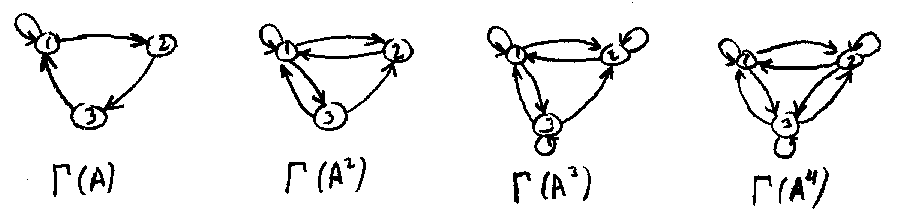
\includegraphics[width=4.5in]{images/GammaIteration.ps}}
\caption{Graphs associated with powers of $A$ defined in \eqref{eqn:AforGammaIteration}}.
\label{fig:GammaIteration}
\end{figure}

\medskip
\noindent
\textbf{Irreducible Matrices and $\Gamma(A)$.}
We give the interpretation of the reducibility of $A$ in terms of the graph $\Gamma(A)$
in the following theorem.

\begin{theorem}
The matrix $A$ is reducible if and only if $\,\Gamma(A)$ contains a subset
$V$ of vertices such that the
edges between $V$ and vertices not in $V$
are all directed out of $V$.
\end{theorem}

\begin{xexample}
We consider the matrix
\begin{equation}
    A = \begin{bmatrix}
             2 & 1 & 1 & 1\\
             0 & 0 & 0 & 1/2 \\
             2 & 1/2 & 1 & 0 \\
             0 & 1 & 0 & 5
        \end{bmatrix}
\label{eqn:AforgraphexampleII}
\end{equation}
The graph $\Gamma(A)$ is shown in Figure~\ref{fig:graphexampleII}.
All the edges from the set $V = \{\textbf{2},\textbf{4}\}$
to $\{\textbf{1},\textbf{3}\}$ are directed out of $V$.
This implies that $A$ is reducible.
This also suggests that the permutation
matrix $P$ that converts $A$ into the reduced block structure
should simply interchange the labels of vertices
$\textbf{2}$ and $\textbf{3}$.  Indeed, if we define
\begin{equation}
   P = \begin{bmatrix}
            1 & 0 & 0 & 0 \\
            0 & 0 & 1 & 0 \\
            0 & 1 & 0 & 0 \\
            0 & 0 & 0 & 1
       \end{bmatrix}
\end{equation}
we find
\begin{equation}
  P^{\textsf{T}}AP = 
      \begin{bmatrix}
              2 & 1 & 1 & 1 \\
              2 & 1 & 1/2 & 0 \\
              0 & 0 & 0 & 1/2 \\
              0 & 0 & 1 & 5
      \end{bmatrix}.
\end{equation}
\end{xexample}

\begin{figure}
\centerline{\includegraphics[width=3.25in]{fig/ExampleGraph2.eps}}
\caption{The graph $\Gamma(A)$ associated with the matrix $A$ defined
in \eqref{eqn:AforgraphexampleII}.}
\label{fig:graphexampleII}
\end{figure}


Irreducibility of $A$ is associated with the degree of ``connectedness''
of the graph of $A$. We shall not need the following definition and
theorem, but they are included for completeness.

\begin{definition}
A directed graph $\Gamma$ is \emph{strongly connected}\index{strongly connected graph}
if there is a directed path from each vertex to all other vertices.
\end{definition}
\begin{theorem}
The $m\times m$ matrix $A$ is irreducible if and only if $\Gamma(A)$
is strongly connected.
\end{theorem}

\newpage
\begin{exercises}
\begin{exercise}
Show that
\begin{equation}
   A = \begin{bmatrix}
                0 & 1 & 0 & 1 \\
                0 & 1 & 0 & 0 \\ 1 & 0 & 0 & 1 \\ 1 & 0 & 1 & 0
       \end{bmatrix}
\end{equation}
is reducible.  Find the permutation matrix $P$ such that $P^{\textsf{T}}AP$
has the block structure shown in \eqref{eqn:reducibleblockstructure}.
Sketch $\Gamma(A)$, and indicate the subset of the vertices
that correspond to the decoupled variables.
\end{exercise}
\end{exercises}
%
\newpage
%
\section{Stochastic Matrices}
Consider the following situation.
There are three cities \textbf{A}, \textbf{B}, and \textbf{C}, initially with
populations of 25,000, 25,000 and 50,000, respectively.
Each year, 5\% of the population of \textbf{A} moves to \textbf{B}
and 10\% of the population of \textbf{A} moves to \textbf{C}.
At the same time, 1\% of the population of \textbf{B} moves to \textbf{C},
and 5\% of the population of \textbf{C} moves to \textbf{A}.
We'll assume that the total population remains constant.

Let $\BX(n) \in \Real^{3}$ represent the population of the three cites
in year $n$, measured in thousands.  Then
\begin{equation}
   \BX(0)=\begin{bmatrix} 25 \\ 25 \\ 50 \end{bmatrix},
\end{equation}
and each year the populations change according to
\begin{equation}
\begin{split}
    x_1(n+1) & = 0.85 x_1(n) + 0.05x_3(n) \\
    x_2(n+1) & = 0.05x_1(n) + 0.99x_2(n)  \\
    x_3(n+1) & = 0.1x_1(n) + 0.01x_2(n) + 0.95x_3(n)
\end{split}
\end{equation}
or
\begin{equation}
    \BX(n+1) = A\BX(n),
\label{eqn:stoch:linmap}
\end{equation}
where
\begin{equation}
    A = \begin{bmatrix}
             0.85 & 0 & 0.05 \\
             0.05  & 0.99 & 0 \\
             0.1 & 0.01 & 0.95
        \end{bmatrix}
\end{equation}
What will be the long-term distribution of the populations?
Will the population of any city approach 0?
We can answer these questions using the tools we have already
derived.

We first observe that $A^2 > 0$.  By the Perron-Frobenius
Theorem for Primitive Matrices, we know that $A$ has
a real, positive, dominant eigenvalue, with a positive eigenvector.
From the discussion in the previous section, we know that
in the long-term, the contribution of $\lambda_1^n\BV_1$ will
dominate the solution.
Of course, we still have to do the work to find this eigenvalue
and eigenvector.

A calculation shows that the eigenvalues of $A$
(in order of decreasing magnitude) are
$\lambda_1 = 1$, $\lambda_2 \approx 0.9758$ and $\lambda_3 \approx 0.8142$.
Since $|\lambda_2| < \lambda_1$ and $|\lambda_3| < \lambda_1$, in the
long-term the solution to \eqref{eqn:stoch:linmap}
will look like
\begin{equation}
   \BX(n) \approx c_1 \lambda_1^n\BV_1 = c_1 \BV_1 
\end{equation}
where $\BV_1$ is an eigenvector associated with $\lambda_1$.
(Since $\lambda_1=1$, we used $\lambda_1^n=1$.)  This says that the
population will approach a consant distribution in the long-term.
Further calculation shows that
\begin{equation}
  \BV_1 = \begin{bmatrix}
               1 \\ 5 \\ 3
          \end{bmatrix}
\end{equation}
Moreover, since the total population remains constant at 100,000,
the entries of $\BX(n)$ must add up to 100, and this must hold in
the long-term.  This implies $c_1(1+5+3) = 100$, or
$c_1 = 100/9$.  Thus, in the long-term, the population approaches
\begin{equation}
    100\begin{bmatrix} 1/9 \\ 5/9 \\ 1/3\end{bmatrix}
\end{equation}
In other words, in the long-term, $1/9$ of the population will
be in \textbf{A}, $5/9$ in \textbf{B} and $1/3$ in \textbf{C}.

Note that the columns of $A$ add up to 1.  This class of matrices
is important enough to have its own name.
\begin{definition}
An $m\times m$ matrix $A$ is called \emph{stochastic}\index{stochastic matrix}
if $A \ge 0$ and the sum of the entries
of each column of $A$ is one.
(Such a matrix is also called a \emph{Markov matrix}.\index{Markov matrix})
\end{definition}
\begin{xexample}
The following matrices are stochastic:
\begin{equation}
  A = \begin{bmatrix}
          0.9 & 0.2 \\ 0.1 & 0.8
      \end{bmatrix},
  \quad
  B = \begin{bmatrix}
          0 & 1 & 0.2 \\ 0.5 & 0 & 0.2 \\ 0.5 & 0 & 0.6
      \end{bmatrix}
\label{eqn:stoch:examples}
\end{equation}
\end{xexample}
In our example of the populations of the three cities,
we found that $1$ was an eigenvalue of the matrix $A$, and it
had a positive eigenvector.  This is true in general.
\begin{theorem}
Let $A$ be a stochastic matrix. Then
\begin{enumerate}
\item $\lambda_1 = 1$ is an eigenvalue of $A$,
and this eigenvalue has a positive eigenvector.
\item $|\lambda_j| \le 1$ for all eigenvalues $\lambda_j$.
\end{enumerate}
\end{theorem}
%
%\emph{Partial Proof.}
Let's look at two proofs of the statement that
$\lambda_1=1$ is an eigenvalue of $A$.

\emph{Proof that $\lambda_1=1$ is an eigenvalue, version 1:}
Since the sums of the columns of $A$ are all $1$,
the sums of the columns of $A-I$ are all $0$.
This implies that the rows of $A-I$ are linearly
dependent, which then implies that
$A-I$ is singular.  This is precisely the condition
for $1$ to be an eigenvalue of $A$.

\emph{Proof that $\lambda_1=1$ is an eigenvalue, version 2:}
Let
\begin{equation}
   \BE = \begin{bmatrix} 1 \\ 1 \\ \vdots \\ 1\end{bmatrix}
\end{equation}
Then it is easily verified that
\begin{equation}
  A^{\textsf{T}}\BE = \BE
\end{equation}
which shows that $1$ is an eigenvalue of $A$, with
eigenvector $\BE$.
Since, in general, $A$ and $A^{\textsf{T}}$ have the
same eigenvalues, $1$ is also an eigenvalue of $A$.
\hfill $\qed$

Before proving that all the eigenvalues of a stochastic
matrix have magnitude less than or equal to $1$, we
define some convenient notation.

\begin{definition}
We define the ``1-norm''\index{1-norm} of an $m$-dimensional vector
$\BX$, written
$\|\BX\|_1$.  The definition is
\begin{equation}
  \| \BX \|_1 = |x_1| + |x_2| + \cdots + |x_m|.
\end{equation}
\end{definition}
The 1-norm is, in fact, a \emph{norm},\index{norm} because it
satisfies these properties:
\begin{enumerate}
\item $\|\BX\|_1 \ge 0$, and $\|\BX\|_1 = 0$ if and only
if $\BX = \BZero$.
\item $\|\lambda \BX\|_1 = |\lambda|\|\BX\|_1$ for any
scalar $\lambda$.
\item $\|\BX+\BY\|_1 \le \|\BX\|_1 + \|\BY\|_1$
(the triangle inequality).\index{triangle inequality}
\end{enumerate}

We'll use the 1-norm in the following.

\emph{Proof that $|\lambda_j|\le 1$ for a stochastic matrix $A$.}
Let $\BU_k$ be the $k$th column of $A$.
By assumption, $\|\BU_k\|_1 = 1$.
We recall from Linear Algebra that
$A\BX$ is a linear combination of the columns of $A$, with
coefficients given by the entries of $\BX$:
\begin{equation}
  A\BX = x_1 \BU_1 + x_2\BU_2 + \cdots + x_m \BU_m.
\end{equation}
Then
\begin{equation}
\begin{split}
  \|A\BX\|_1 & = \|x_1\BU_1 + x_2 \BU_2 + \cdots + x_m\BU_m\|_1 \\
             & \le \|x_1 \BU_1\|_1 + \|x_2 \BU_2\|_1 + \cdots + \| x_m \BU_m\|_1 \\
	     & = |x_1|\|\BU_1\|_1 + |x_2|\|\BU_2\|_1 + \cdots + |x_m|\|\BU_m\|_1 \\
	     & = |x_1| + |x_2| + \cdots + |x_m| \\
	     & = \|\BX\|_1.
\end{split}
\end{equation}
So
\begin{equation}
\|A\BX\|_1 \le \|\BX\|_1
\label{eqn:norminequality}
\end{equation}
for any $\BX$.  If
\begin{equation}
  A\BX = \lambda \BX,
\end{equation}
then \eqref{eqn:norminequality} implies
\begin{equation}
  \|\lambda\BX\|_1 \le \|\BX\|_1,
\end{equation}
and since
\begin{equation}
  \|\lambda \BX\|_1 = |\lambda|\|\BX\|_1,
\end{equation}
we have
\begin{equation}
 |\lambda| \|\BX\|_1 \le \|\BX\|_1
\end{equation}
which implies
\begin{equation}
 |\lambda| \le 1.
\end{equation}
\begin{xexample}
Let $A$ and $B$ be the matrices given in \eqref{eqn:stoch:examples}.
For $A$, we find $\lambda_1 = 1$ and $\lambda_2 = 0.7$.
For $B$, we find $\lambda_1 = 1$,
$\lambda_2 = (-1+\sqrt{6})/5 \approx 0.2899$,
and $\lambda_3 = (-1-\sqrt{6})/5 \approx -0.6899$.
In both cases we find $\lambda_1=1$ and $|\lambda_j|\le 1$, as
required by the theorem.
\end{xexample}
\begin{xexample}
The matrix
\begin{equation}
  P = \begin{bmatrix}
          0 & 1 \\
	  1 & 0
      \end{bmatrix}
\end{equation}
is stochastic. We find that the eigenvalues
are $\lambda_1 = 1$ and $\lambda_2 = -1$.
Note that the magnitude of both eigenvalues is 1.
\end{xexample}
Note that the theorem for stochastic matrices
does not say that the eigenvalue
$\lambda_1 = 1$ is simple.
(Compare the conclusion of that theorem to the
conclusions of the Perron-Frobenius Theorems.)
\begin{xexample}
Let $I$ be the $m\times m$ identity matrix.
The \emph{only} eigenvalue of $I$ is $\lambda_1 = 1$, and it
has multiplicity $m$; the eigenvalue is \emph{not} simple.
\end{xexample}
We will see many more examples of stochastic matrices
in the chaper on Markov Chains.
%

\newpage
\begin{exercises}
\begin{exercise}
Find a $4\times 4$ stochastic matrix with eigenvalues
$1$, $-1$, $i$ and $-i$.
\end{exercise}
\end{exercises}
%
\newpage
%
\section{Age-Structured Populations and Leslie Matrix Models}
\index{Leslie matrix}
\emph{introduction, basic idea, etc...}

We consider a population in which the maximum
age is $m$.
Let $x_{k}(n)$ be the number of individuals
of age $k$ at time $n$.
(We use this notation because
I find $x_{k}(n+1)$
easier to read than $x_{k,n+1}$--or would it be $x_{n+1,k}$?)
Let
$p_k$ be the probability of surviving from age $k$
to age $k+1$,
and let $f_k$ be the number of offspring per individual
of age $k$.
We define $x_0(n)$ to be the number of newborn individuals
in time $n$.
Then
\begin{equation}
  x_{0}(n+1) = f_1 x_{1}(n) + f_2 x_{2}(n) + \cdots + f_m x_{m}(n)
\label{eqn:leslie:newborn}
\end{equation}
Then, for $1 \le k \le m$, we have
\begin{equation}
   x_{k}(n+1) = p_k x_{k}(n),
\label{eqn:leslie:nextgen}
\end{equation}

The ``state'' of this system is the $m+1$ dimensional
vector
\begin{equation}
  \BX(n) = \begin{bmatrix} x_0(n) \\ x_1(n) \\ \vdots \\x_m(n)
           \end{bmatrix}
\end{equation}
and we can combine equations \eqref{eqn:leslie:newborn}
and \eqref{eqn:leslie:nextgen} into the matrix equation
\begin{equation}
   \begin{bmatrix}
      x_0(n+1) \\ x_1(n+1) \\ x_2(n+1) \\ x_3(n+1) \\ \vdots \\x_m(n+1)
   \end{bmatrix}
    =
   \begin{bmatrix}
      f_0 & f_1 &  f_2 & \cdots & f_{m-1} & f_m \\
      p_0 &  0  &   0  &        &  0      &  0  \\
       0  & p_1 &   0  &        &  0      &  0  \\
       0  &  0  &  p_2  &       &  0      &  0  \\
       \vdots & & & \ddots \\
       0 &  0  &   0  & & p_{m-1} & 0 \\
   \end{bmatrix}
   \begin{bmatrix}
       x_0(n) \\ x_1(n) \\ x_2(n) \\ x_3(n) \\ \vdots \\x_m(n)
   \end{bmatrix}
\label{eqn:leslie1}
\end{equation}
or more compactly
\begin{equation}
   \BX(n+1) = A\BX(n)
\end{equation}
where $A$ is the matrix in \eqref{eqn:leslie1}.

Recall that for the simplest population model, $p(n+1) = rp(n)$,
the long-term survival of the population was determined 
by $r$. If $r > 1$, the population would grow exponentially,
and if $0 < r < 1$, the population would decay exponentially.
We can ask the same question for an age-structured population:
Will this population grow or decay?

The answer can be found by determining the eigenvalues
of $\lambda_k$ of $A$.
If for some $k$,  $|\lambda_k| > 1$, then it is possible
that the population will grow.  If, for all eigenvalues,
$|\lambda_k| < 1$, the population will decay to zero
asymptotically.

\medskip
\noindent
\emph{Discuss how, in the long term, the population
distribution is determined by the dominant eigenvalue.}
%
%
\newpage
%
\section{Stage-Structured Lefkovitch Models}
\index{Lefkovitch models}
Leslie models assume that development and maturity
depend only on chronological age.  This is not always
the case.

An alternate model is to consider the specific stages
of development (e.g. egg, larva, pupa, adult, etc).
A graph is developed that represents the possible transitions
among the stages in a single time unit, and the edges
of the graphs are labeled with the multiplicative
factor for that transition.  For example, if in a given
population, 75\% of the eggs survive to form larva,
a transition edge would connect eggs to larva, with
a numerical label of 0.75.

From the transition graph, we obtain a matrix equation
for the populations of each stage.

\emph{etc...}

\noindent
\emph{These models are analyzed using the same techniques
as for the Leslie models.}
%